\documentclass[tikz,border=10pt]{standalone}
\usepackage{tikz}

\definecolor{furMain}{RGB}{212,157,109}
\definecolor{furShade}{RGB}{182,124,78}
\definecolor{furLight}{RGB}{238,205,163}
\definecolor{furOutline}{RGB}{120,78,48}
\definecolor{noseBrown}{RGB}{92,58,38}
\definecolor{blushPink}{RGB}{255,178,158}
\definecolor{patchRed}{RGB}{209,88,66}
\definecolor{patchCream}{RGB}{250,231,178}
\definecolor{eyeBlack}{RGB}{40,30,25}

\begin{document}
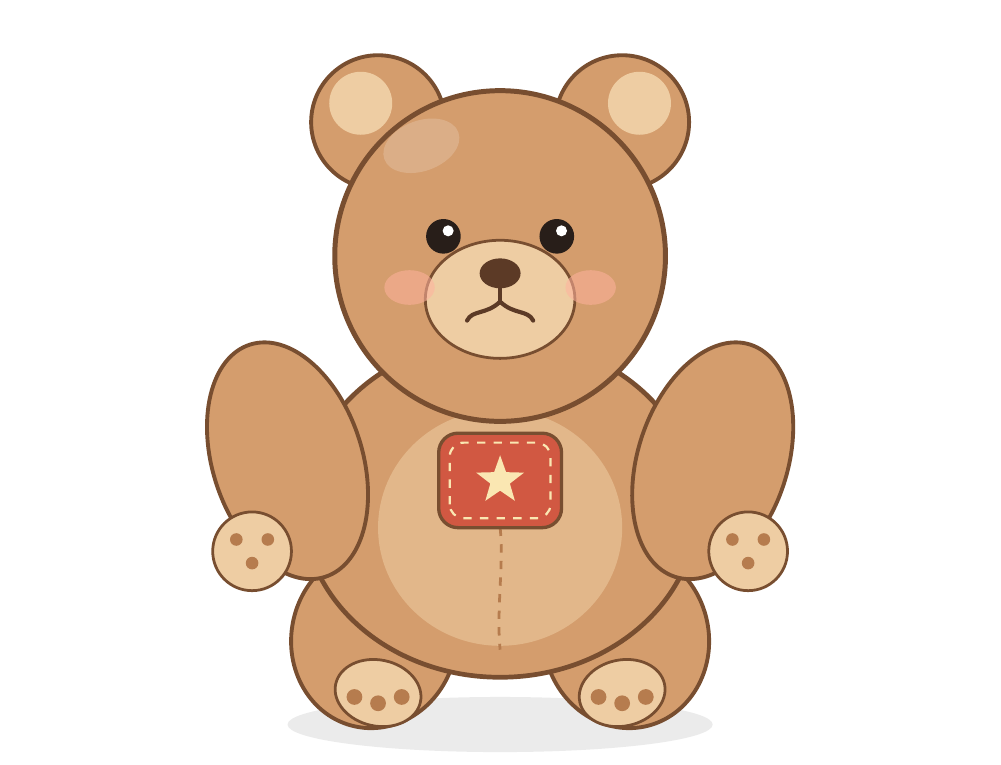
\begin{tikzpicture}[line join=round]

% fixed canvas, 12cm x 9cm (4:3, "1200x900" proportions)
\path[use as bounding box] (-6,-4.5) rectangle (6,4.5);

% soft ground shadow
\fill[black,opacity=0.08] (0,-4.35) ellipse [x radius=2.7,y radius=0.35];

% legs (drawn behind body)
\fill[furMain,draw=furOutline,line width=1.4pt,rotate around={-12:(-1.6,-3.25)}]
  (-1.6,-3.25) ellipse [x radius=1.05,y radius=1.15];
\fill[furMain,draw=furOutline,line width=1.4pt,rotate around={12:(1.6,-3.25)}]
  (1.6,-3.25) ellipse [x radius=1.05,y radius=1.15];

% foot soles with toe beans
\fill[furLight,draw=furOutline,line width=1pt,rotate around={-12:(-1.55,-3.95)}]
  (-1.55,-3.95) ellipse [x radius=0.55,y radius=0.42];
\fill[furShade] (-1.85,-4.0) circle [radius=0.10];
\fill[furShade] (-1.55,-4.08) circle [radius=0.10];
\fill[furShade] (-1.25,-4.0) circle [radius=0.10];

\fill[furLight,draw=furOutline,line width=1pt,rotate around={12:(1.55,-3.95)}]
  (1.55,-3.95) ellipse [x radius=0.55,y radius=0.42];
\fill[furShade] (1.85,-4.0) circle [radius=0.10];
\fill[furShade] (1.55,-4.08) circle [radius=0.10];
\fill[furShade] (1.25,-4.0) circle [radius=0.10];

% body (soft, wide silhouette for a stuffed feel)
\fill[furMain,draw=furOutline,line width=1.7pt] (0,-1.6) ellipse [x radius=2.5,y radius=2.15];

% soft belly shading
\fill[furLight,opacity=0.55] (0,-1.85) ellipse [x radius=1.55,y radius=1.5];

% belly stitch seam below the patch
\draw[furShade,dashed,line width=1pt]
  (0,-1.85) .. controls (0.05,-2.3) and (-0.05,-2.9) .. (0,-3.4);

% chest wappen (appliqu\'e patch) with stitched border and star
\fill[patchRed,draw=furOutline,line width=1.2pt,rounded corners=7pt] (-0.78,-1.85) rectangle (0.78,-0.65);
\draw[patchCream,dashed,line width=0.8pt,rounded corners=5pt] (-0.64,-1.73) rectangle (0.64,-0.77);
\fill[patchCream]
  (0.00,-0.93) -- (-0.076,-1.145) -- (-0.304,-1.151) -- (-0.124,-1.290) --
  (-0.188,-1.509) -- (0.000,-1.380) -- (0.188,-1.509) -- (0.124,-1.290) --
  (0.304,-1.151) -- (0.076,-1.145) -- cycle;

% arms (short, rounded, angled slightly outward)
\fill[furMain,draw=furOutline,line width=1.4pt,rotate around={18:(-2.7,-1.0)}]
  (-2.7,-1.0) ellipse [x radius=0.95,y radius=1.55];
\fill[furMain,draw=furOutline,line width=1.4pt,rotate around={-18:(2.7,-1.0)}]
  (2.7,-1.0) ellipse [x radius=0.95,y radius=1.55];

% paw pads
\fill[furLight,draw=furOutline,line width=1pt] (-3.15,-2.15) circle [radius=0.5];
\fill[furShade] (-3.35,-2.0) circle [radius=0.08];
\fill[furShade] (-2.95,-2.0) circle [radius=0.08];
\fill[furShade] (-3.15,-2.3) circle [radius=0.08];

\fill[furLight,draw=furOutline,line width=1pt] (3.15,-2.15) circle [radius=0.5];
\fill[furShade] (2.95,-2.0) circle [radius=0.08];
\fill[furShade] (3.35,-2.0) circle [radius=0.08];
\fill[furShade] (3.15,-2.3) circle [radius=0.08];

% ears: outer + inner drawn before the head, so the head trims them cleanly
\fill[furMain,draw=furOutline,line width=1.4pt] (-1.55,3.3) circle [radius=0.85];
\fill[furLight] (-1.77,3.54) circle [radius=0.4];
\fill[furMain,draw=furOutline,line width=1.4pt] (1.55,3.3) circle [radius=0.85];
\fill[furLight] (1.77,3.54) circle [radius=0.4];

% head
\fill[furMain,draw=furOutline,line width=1.8pt] (0,1.6) circle [radius=2.1];

% gentle head shine
\fill[white,opacity=0.18,rotate around={20:(-1.0,3.0)}] (-1.0,3.0) ellipse [x radius=0.5,y radius=0.32];

% muzzle
\fill[furLight,draw=furOutline,line width=1pt] (0,1.05) ellipse [x radius=0.95,y radius=0.75];

% eyes
\fill[eyeBlack] (-0.72,1.85) circle [radius=0.22];
\fill[white] (-0.66,1.92) circle [radius=0.07];
\fill[eyeBlack] (0.72,1.85) circle [radius=0.22];
\fill[white] (0.78,1.92) circle [radius=0.07];

% cheek blush
\fill[blushPink,opacity=0.55] (-1.15,1.2) ellipse [x radius=0.32,y radius=0.22];
\fill[blushPink,opacity=0.55] (1.15,1.2) ellipse [x radius=0.32,y radius=0.22];

% nose
\fill[noseBrown] (0,1.38) ellipse [x radius=0.26,y radius=0.19];

% mouth
\draw[noseBrown,line width=1.5pt,line cap=round] (0,1.19) -- (0,1.02);
\draw[noseBrown,line width=1.5pt,line cap=round]
  (0,1.02) .. controls (-0.18,0.85) and (-0.35,0.92) .. (-0.42,0.78);
\draw[noseBrown,line width=1.5pt,line cap=round]
  (0,1.02) .. controls (0.18,0.85) and (0.35,0.92) .. (0.42,0.78);

\end{tikzpicture}
\end{document}
